% Vista preliminar del código fuente

%% LyX 2.0.0 created this file.  For more info, see http://www.lyx.org/.
%% Do not edit unless you really know what you are doing.
\documentclass[english]{article}
\usepackage[T1]{fontenc}
\usepackage[latin9]{inputenc}
\usepackage[a4paper]{geometry}
\geometry{verbose,tmargin=2cm,bmargin=3cm,lmargin=2cm,rmargin=2cm}
\usepackage{array}
\usepackage{float}
\usepackage{multirow}
\usepackage{amssymb}
\usepackage{graphicx}

\makeatletter

%%%%%%%%%%%%%%%%%%%%%%%%%%%%%% LyX specific LaTeX commands.
%% Because html converters don't know tabularnewline
\providecommand{\tabularnewline}{\\}

%%%%%%%%%%%%%%%%%%%%%%%%%%%%%% Textclass specific LaTeX commands.
\newenvironment{lyxcode}
{\par\begin{list}{}{
\setlength{\rightmargin}{\leftmargin}
\setlength{\listparindent}{0pt}% needed for AMS classes
\raggedright
\setlength{\itemsep}{0pt}
\setlength{\parsep}{0pt}
\normalfont\ttfamily}%
 \item[]}
{\end{list}}

\makeatother

\usepackage{babel}
\begin{document}

\title{Aprendizaje Automático - Trabajo Práctico 4}


\author{Gonzalo Castiglione - 49138}

\maketitle

\paragraph*{Objetivo: Aprender a agrupar datos mediante análisis de clusters}


\section{Determinación de clases. Clustering.}
\begin{enumerate}
\item Una consideracion a tener antes del cálculo de las componentes principales
es que las unidades de medida de las variables $X_{i}$ son muy distintas
y no hay que olvidar que los cambios de unidades afectan a la varianza
de la variable en el sentido que: 
\[
\xi=aX_{i}\Longrightarrow var(\xi)=a^{2}var(X_{i})
\]
 y como consecuencia, esto afecta a las componentes principales.


Las elevadas varianzas de las mediciones de {}``Número de teléfonos
fijos registrados'' y el {}``Número de vehículos de motor matriculados''
hacen prever que un análisis de componentes principales realizado
a partir de la matriz de covariansa $S$ dará como resultado una primera
y segunda componentes principales que coincidan basicamente con estas
dos variables observadas.


Para poder obtener componentes principales que no dependan de las
unidades en que han sido medidas las variables originales, se debe
estandarizar a media cero y varianza uno las variables originales.
Lo que equivale a realizar el análisis de componentes a partir de
la matriz de correlaciones. Para esto se utiliza el comando de $matlab$
princomp que tiene en cuanta estos detalles.
\begin{enumerate}
\item A partir del anális de las componentes principales, se puede ver que
basta tomar una sola componente para clasificas a las provincias dado
que ya se tiene una representacion muy precisa de las muestras.


\begin{center}
\begin{tabular}{|c|c|}
\hline 
 & $\%$\tabularnewline
\hline 
\hline 
1 & $0.9961$\tabularnewline
\hline 
2 & $0.999$\tabularnewline
\hline 
3 & $1$\tabularnewline
\hline 
4 & ...\tabularnewline
\hline 
\end{tabular}
\par\end{center}


En este caso, con la variable población es suficiente para clasificar
la muestra en un $99\%$.


\begin{center}
\begin{figure}[H]
\centering{}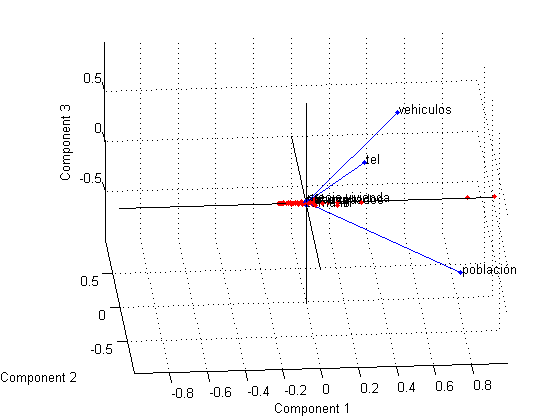
\includegraphics[scale=0.5]{ciudadesEspañolas1}\caption{Biplot de las componentes de las mediciones para las mediciones de
las ciudades españolas}
\end{figure}

\par\end{center}

\item %
\begin{tabular}{|c||c|c|c|c|}
\hline 
\multicolumn{1}{|c|}{} & \multicolumn{2}{c|}{A(2)} & \multicolumn{2}{c|}{B(15)}\tabularnewline
\hline 
Variable & Media & Varianza & Media & Varianza\tabularnewline
\hline 
\hline 
Poblacion & 5,595,248.5  & 521,695.605 & 1,262,343.867  & 430,782.681 \tabularnewline
\hline 
Tel. Fijo & 2,802,510.5  & 88,271.675 & 475,434.6  & 155,222.802\tabularnewline
\hline 
Vehiculos Matriculados & 346,810  & 423,110.070  & 748,407.267  & 272,113.378\tabularnewline
\hline 
\end{tabular}


\begin{tabular}{|c||c|c|}
\hline 
\multicolumn{1}{|c|}{} & \multicolumn{2}{c|}{C(35)}\tabularnewline
\hline 
Variable & Media & Varianza\tabularnewline
\hline 
\hline 
Poblacion & 399,510.714  & 207,726.956\tabularnewline
\hline 
Tel. Fijo & 157,819.943  & 83,126.300\tabularnewline
\hline 
Vehiculos Matriculados & 237,011.257  & 124,416.649\tabularnewline
\hline 
\end{tabular}


Resulta de interés resaltar que para los dos miembros de la clase
$A$, sus varianzas superan en las de cinco veces la de la clase $B$
y en mucho mas la de la $C$. Por lo que se podría realizar un nuevo
análisis de los datos removiendo estos dos valores y analizando nuevamente
los nuevos grupos formados.

\end{enumerate}
\item Lirios de Fisher

\begin{enumerate}
\item Clasificación del las mediciónes según el algoritmo $kmeans$


\begin{center}
\begin{figure}[H]
\begin{centering}
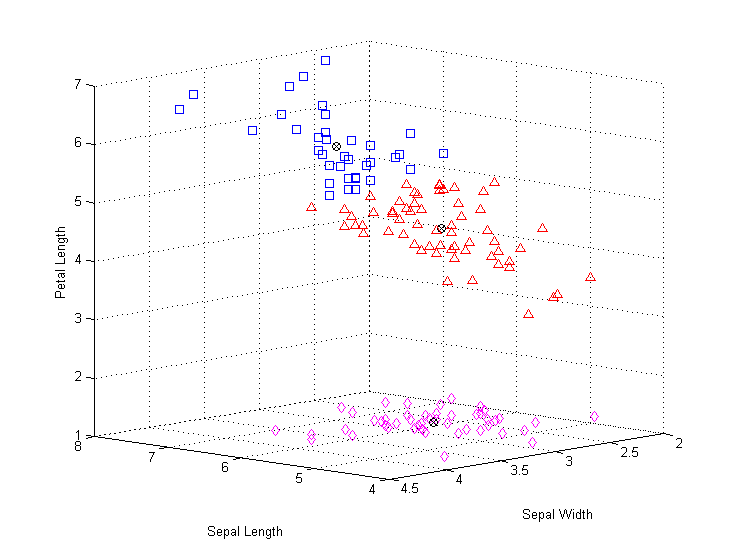
\includegraphics[scale=0.5]{kmeans2}\caption{Agrupamiento de los lirios de Fisher}

\par\end{centering}

\end{figure}

\par\end{center}


Matriz de confusión


\begin{center}
\begin{tabular}{|c|c|c|c|c|}
\hline 
 & \multicolumn{4}{c|}{Clase Predicha}\tabularnewline
\hline 
\multirow{4}{*}{Clase Real} &  & Setosa & Versicolor & Virginica\tabularnewline
\cline{2-5} 
 & Setosa & $50$ & $0$ & $0$\tabularnewline
\cline{2-5} 
 & Versicolor & $0$ & $42$ & $8$\tabularnewline
\cline{2-5} 
 & Virginica & $0$ & $14$ & $36$\tabularnewline
\hline 
\end{tabular}
\par\end{center}


\[
error=\frac{8+14}{150}\backsimeq0.15
\]


\item Calsificación segun algoritmo de clusters jerárquicos aglomerativos


\begin{center}
\begin{figure}[H]
\centering{}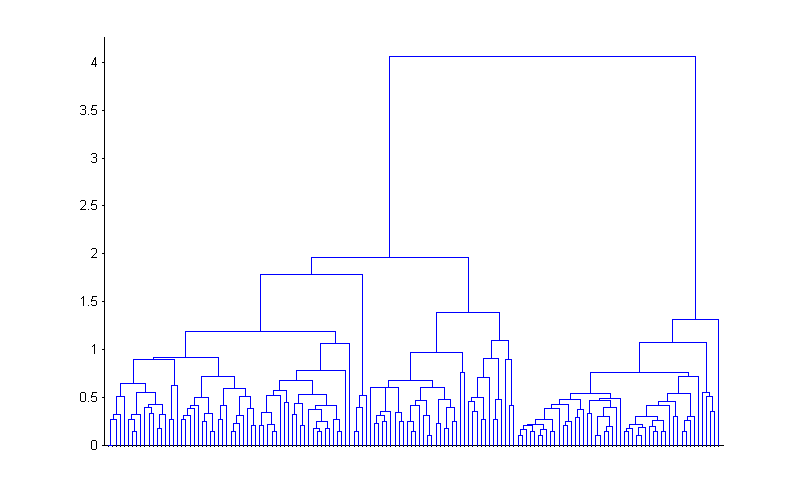
\includegraphics[scale=0.5]{liriosFisher}\caption{Agrupamiento de los lirios de Fisher}
\end{figure}

\par\end{center}


Matriz de confusión


\begin{center}
\begin{tabular}{|c|c|c|c|c|}
\hline 
 & \multicolumn{4}{c|}{Clase Predicha}\tabularnewline
\hline 
\multirow{4}{*}{Clase Real} &  & Setosa & Versicolor & Virginica\tabularnewline
\cline{2-5} 
 & Setosa & $50$ & $0$ & $0$\tabularnewline
\cline{2-5} 
 & Versicolor & $0$ & $49$ & $1$\tabularnewline
\cline{2-5} 
 & Virginica & $0$ & $15$ & $35$\tabularnewline
\hline 
\end{tabular}
\par\end{center}


\[
error=\frac{1+15}{150}\backsimeq0.11
\]


\item Luego de comprados los resultados obtenidos por cada algoritmo en
los puntos $(a)$ y $(b)$ se pudo concluir que para este problema,
el algoritmo que mejor clasifica a los los lirios recogidos es el
de clasificación jerarquica ya que obtuvo un error menor al momento
de realizar las clasificaciones.


Matriz obtenida en el ejercicio $5$ del tp $2$:


\begin{center}
\begin{tabular}{|c|c|c|c|c|}
\hline 
 & \multicolumn{4}{c|}{Clase Predicha}\tabularnewline
\hline 
\multirow{4}{*}{Clase Real} &  & Setosa & Versicolor & Virginica\tabularnewline
\cline{2-5} 
 & Setosa & $50$ & $0$ & $0$\tabularnewline
\cline{2-5} 
 & Versicolor & $0$ & $47$ & $3$\tabularnewline
\cline{2-5} 
 & Virginica & $0$ & $3$ & $47$\tabularnewline
\hline 
\end{tabular}
\par\end{center}


\[
error=\frac{3+3}{150}\backsimeq0.04
\]



Como se pudo obervar, este algoritmo clasificó aun mejor que los anteriores
a los lirios, en especial para los de la clase $Virginica$, que es
donde mayor cantidad de errores tuvieron los dos anteriores.

\end{enumerate}
\item Dialectos ingleses

\begin{enumerate}
\item A continuación se presentan los gráficos obtenidos para diversos parámetros
de distancia y método de agrupamiento de datos para el dendograma


\begin{figure}[H]
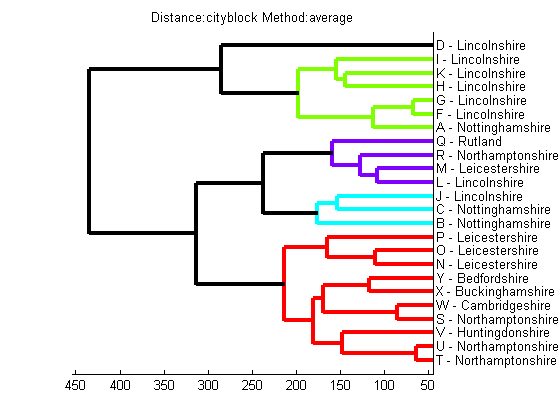
\includegraphics[scale=0.55]{dialects1}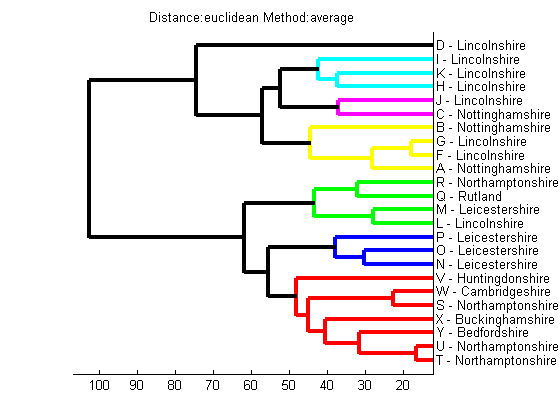
\includegraphics[scale=0.55]{dialects4}

\caption{Método: $average$ para distancias $euclidean$ y $cityblock$}


\end{figure}



\begin{figure}[H]
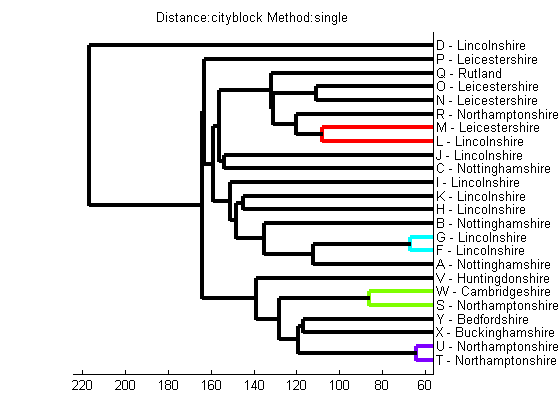
\includegraphics[scale=0.55]{dialects3}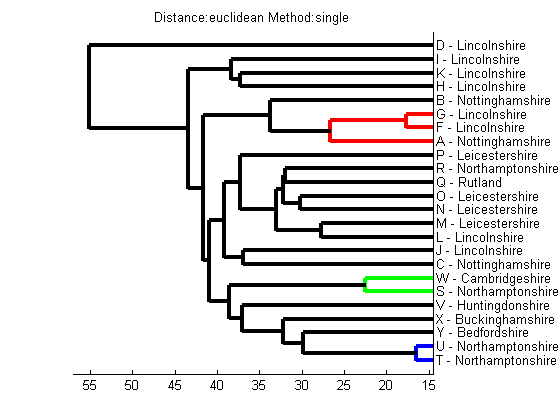
\includegraphics[scale=0.55]{dialects6}

\caption{Método: $signle$ para distancias $euclidean$ y $cityblock$}
\end{figure}



\begin{figure}[H]
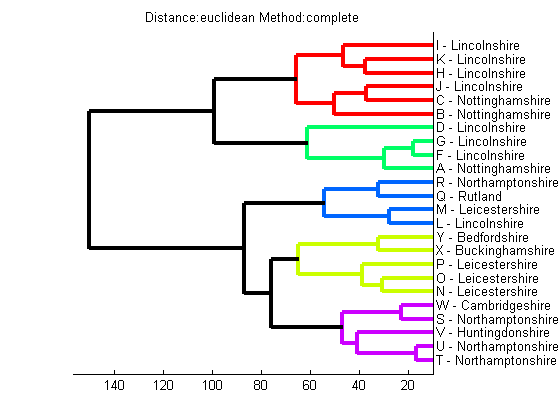
\includegraphics[scale=0.55]{dialects5}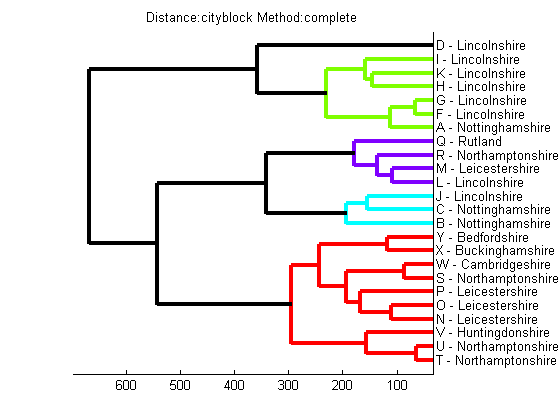
\includegraphics[scale=0.55]{dialects2}

\caption{Método: $complete$ para distancias $euclidean$ y $cityblock$}
\end{figure}



De los resultados obtenidos se puede observar que los métodos $avergae$
y $complete$ son los que mas parecidos agruparon a los condados (para
ambos tipos de distancias).\\


\end{enumerate}
\item Congresistas

\begin{enumerate}
\item Luego de realizadas pruebas de clasificación variando el tipo de distancia
entre $euclidean$ y $cityblock$. Y el tipo de metodo de creación
del árbol jerárquico entre $single$, $complete$ y $average$. Se
pudo observar que todos pudieron calsificar correctamente a todos
los congrsistas de acuerdo a si es Demócrata o Republicando (excepto
por uno que siempre es clasificado mal) a excepción del método $single$,
el cual terminó por clasificar a todos como Democratas excepto por
el número $2$, que fue clasificado correctamente con Republicano.
\end{enumerate}

\begin{center}
\begin{figure}[H]
\centering{}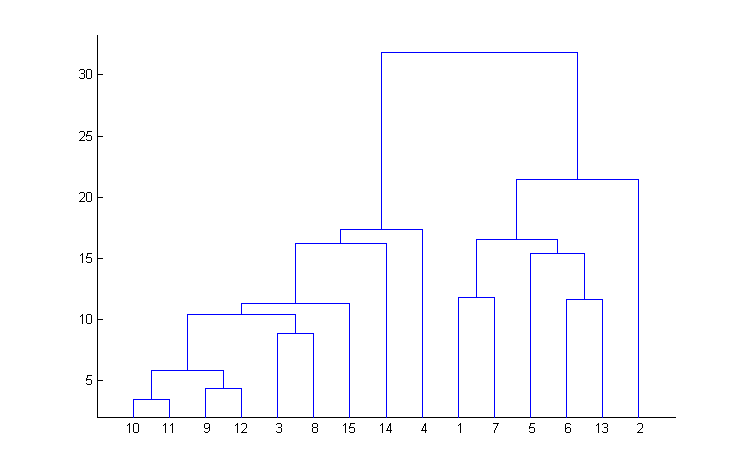
\includegraphics[scale=0.4]{Congresistas_euc_avg}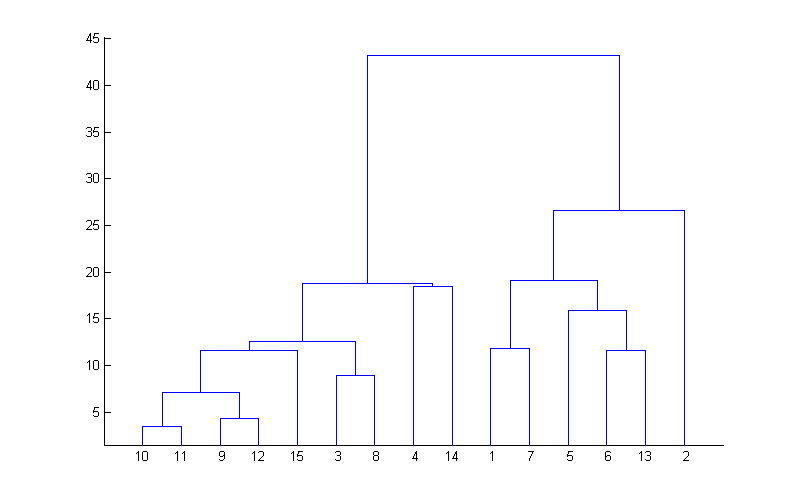
\includegraphics[scale=0.4]{Congresistas_euc_comp}\caption{Árbol de jerarqua creados utilizando al distancia $euclidea$ con
el método $average$(izquierda) y el método $complete$(derecha)}
\end{figure}

\par\end{center}


\begin{center}
Para los métodos aplicados en los gráficos anteriores, se puede observar
que si bien se obtuvieron distintas categorías para varios conjuntos
de congresistas, tomando clusters de $2$ (por los grupos democrata
o republicano) ambos algoritmos clasificaron correctamente a todos
los congresistas a exepción del numero $12$ que en realidad pertenece
al partido republicano.
\par\end{center}


A continuación se muestra la matriz de confusión para ambos árboles
jerarquicos (notar que ambos presentan la misma matriz):\\



\begin{center}
\begin{tabular}{|c|c|c|c|}
\hline 
 & \multicolumn{3}{c|}{Clase Predicha}\tabularnewline
\hline 
\multirow{3}{*}{Clase Real} &  & Demócrata & Republicano\tabularnewline
\cline{2-4} 
 & Demócrata & $8$ & $1$\tabularnewline
\cline{2-4} 
 & Republicano & $0$ & $6$\tabularnewline
\hline 
\end{tabular}
\par\end{center}


\[
error=\frac{1}{15}\backsimeq0.07
\]



\begin{center}
\begin{figure}[H]
\centering{}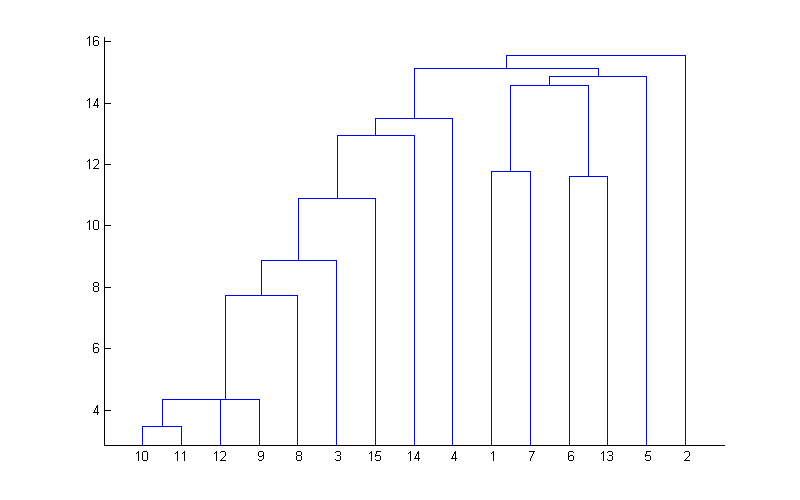
\includegraphics[scale=0.4]{Congresistas_euc_sin}\caption{Árbol de jerarqua creado utilizando al distancia $euclidea$ con el
método $single$}
\end{figure}

\par\end{center}


Como se puede ver en la figura 4, no se obtuvieron buenos resultados
al tratar de utilizar el metodo $single$ (minimas distancias) para
agrupar los datos ya que fueron clasificados todos dentro de la misma
categoria, a excepcion del numero 2.

\end{enumerate}
\newpage{}


\section{Código}
\begin{enumerate}
\item Ciudades españolas

\begin{lyxcode}
{[}coeff,~score,~latent{]}~=~princomp(ciudadesEspanolas);

cumsum(latent)./sum(latent)

biplot(coeff,'scores',~score,~'varlabels',~nombres)

-{}-{}-{}-{}-{}-{}-{}-{}-{}-{}-{}-{}-{}-{}-{}-{}-{}-{}-

X~=~kmeans(ciudadesEspanolas,~2);

k~=~1;

nombres(find(X~==~k))

mean(ciudadesEspanolas(find(X~==~k),1))
\end{lyxcode}
\item Lirios de Fisher

\begin{lyxcode}
//~a)

ptsymb~=~\{'bs','r\textasciicircum{}','md','go','c+'\};

load~fisheriris;

k~=~3;

{[}cidx,cmeans,sumd{]}~=~kmeans(meas,k);

for~i~=~1:k
\begin{lyxcode}
clust~=~find(cidx==i);

plot3(meas(clust,1),~meas(clust,2),~meas(clust,3),~ptsymb\{i\});

hold~on
\end{lyxcode}
end~

plot3(cmeans(:,1),~cmeans(:,2),~cmeans(:,3),'ko');~

plot3(cmeans(:,1),~cmeans(:,2),~cmeans(:,3),'kx');

hold~off

xlabel('Sepal~Length');

ylabel('Sepal~Width');

zlabel('Petal~Length');

view(-137,10);

grid~on



types~=~{[}ones(1,50){*}2~ones(1,50)~ones(1,50){*}3{]};

cMat~=~confusionmat(types,cidx)



//~b)

dist~=~pdist(meas,~'euclidean');

clustTree~=~linkage(dist,~'average');

{[}h,~nodes{]}~=~dendrogram(clustTree);

set(gca,~'TickDir',~'out',~'TickLength',~{[}.002~0{]},~'XTickLabel',~{[}{]});





cluster\_labels~=~cluster(clustTree,~'maxclust',~3~);~

confusion\_matrix~=~crosstab(~cluster\_labels,~class~)~
\end{lyxcode}
\item -

\begin{lyxcode}
dialects=load('dialects.mat');

dialects=dialects.A\_pastespecial;

labels=\{'A~-~Nottinghamshire','B~-~Nottinghamshire','C~-~Nottinghamshire',...~~~~~

'D~-~Lincolnshire','F~-~Lincolnshire','G~-~Lincolnshire','H~-~Lincolnshire',...~~~~~

'I~-~Lincolnshire','J~-~Lincolnshire','K~-~Lincolnshire','L~-~Lincolnshire',...~~~~~

'M~-~Leicestershire','N~-~Leicestershire','O~-~Leicestershire',...~~~~~

'P~-~Leicestershire','Q~-~Rutland','R~-~Northamptonshire',...~~~~~

'S~-~Northamptonshire','T~-~Northamptonshire','U~-~Northamptonshire',...~~~~~

'V~-~Huntingdonshire','W~-~Cambridgeshire','X~-~Buckinghamshire',~...

'Y~-~Bedfordshire'\};

methods=\{'single','complete','average'\};~

distances=\{'euclidean','cityblock'\};

for~i=1:size(distances,2)~~~~~
\begin{lyxcode}
distance=distances\{i\};~~~~~

for~j=1:size(methods,2)~~~~~~~~~
\begin{lyxcode}
method=methods\{j\};~~~~~~~~~

thistitle=strcat('Distance:',~distance,'~Method:~',method);~~~~~~~~~~~~~~~~~~~~~~~~~~~~Y=pdist(dialects,distance);~~~~~~~~~

Z=linkage(Y,method);~~~~~~~~~

t~=~.5{*}(max(Z(:,3)));~\%~dendogram~plot~threshold~~~~~~~~~

figure;{[}H,T{]}~=~dendrogram(Z,'colorthreshold',t,'labels',~...

labels,~'Orientation','left');~~~~~~~~~

set(H,'LineWidth',3)~~~~~~~~~

title(thistitle);~~~~~
\end{lyxcode}
end~
\end{lyxcode}
end
\end{lyxcode}
\item Congresistas

\begin{lyxcode}
Y~=~pdist(X,~'cityblock');

Z~=~linkage(Y,~'average');

H~=~dendrogram(Z);
\end{lyxcode}
\end{enumerate}
\begin{lyxcode}
\end{lyxcode}

\end{document}
